\documentclass{article}
\usepackage[utf8]{inputenc}
\usepackage[T1]{fontenc}
\usepackage[left=20mm,top=25mm,right=30mm,bottom=20mm]{geometry}
\usepackage[croatian]{babel}
\usepackage{amsmath}
\usepackage{fix-cm}
\usepackage{hyperref}
\usepackage{enumerate}
\usepackage{graphicx}
\usepackage{multicol}
\usepackage{multirow}
\usepackage{listings}
\usepackage{tikz}
\usepackage{circuitikz}
\usetikzlibrary{arrows,shapes,automata,backgrounds,petri,patterns,shadows,fadings,calc,decorations,decorations.text,circuits.logic.US}
\usepackage{array}
\usepackage{pgfplots}
\usetikzlibrary{calc} 
\usepackage{calc}
\usepackage{pdfpages}
\usepackage{embedfile}
\usepackage{color}
\usepackage{colortbl}
\usepackage{fancyhdr}
\usepackage[shadow,color=mycolor,linecolor=mycolor,bordercolor=black,textwidth=24mm]{todonotes}
\definecolor{mycolor}{RGB}{245,204,204}
\definecolor{mycolor1}{RGB}{194,42,20}
\definecolor{mycolor2}{RGB}{204,255,204}
\definecolor{mycolor3}{RGB}{204,204,255}
\definecolor{mycolor4}{RGB}{255,229,204}
\definecolor{mycolor5}{RGB}{255,204,204}
\definecolor{tablecolor}{RGB}{76,76,76}
\definecolor{parcolor}{RGB}{235,229,229}
\definecolor{tamnozelena}{RGB}{0,155,0}

\newcommand{\plavo}[1]
{\texttt{\color{blue}#1\color{black}}~}
 
\newcommand{\crveno}[2]
{\texttt{\color{red}#1\color{black}}~}

\newcommand{\blokfont}[1]
{\ssfamily{\tiny{\textbf{\color{white}#1\color{black}}}}~}


\hypersetup{
colorlinks,
citecolor=black,
filecolor=black,
linkcolor=black,
urlcolor=black,
}

\setlength{\headheight}{12pt}
\fancypagestyle{logo_stil}
{
\lhead{\small\sc{Omerović Lejla}} \chead{} \rhead{\includegraphics[scale=0.05,trim=0.25mm 0.25mm 0.25mm 0.25mm,clip=true]{logo.pdf}}
\lfoot{} \cfoot{\thepage} \rfoot{}
\renewcommand{\headrulewidth}{0.35pt}
\renewcommand{\footrulewidth}{0pt}}
\renewcommand{\arraystretch}{1.3}
\newcommand{\newsize}[1]{\fontsize{8pt}{21pt}\selectfont{#1}}
\newcommand{\newtodo}[1]{\todo{\newsize{#1}}}
\addto\captionscroatian{\renewcommand{\figurename}{Sličica}}
\addto\captionscroatian{\renewcommand{\tablename}{Tabelica}}
\addto{\captionscroatian}{\renewcommand{\abstractname}{Abstract}}
\addto\captionscroatian{\renewcommand{\listfigurename}{Lista slika}}
\addto\captionscroatian{\renewcommand{\listtablename}{Lista tabela}}

\setlength\parindent{0pt} %iskljuceno uvlacenje za cijeli dokument

\begin{document}
\setcounter{page}{1}
\noindent Univerzitet u Tuzli \hfill{} PROLJEĆE 2020\\
\noindent Fakultet elektrotehnike \hfill{} {Omerović Lejla}\\
\noindent Tehnologije za podršku tehničkom pisanju
\vspace{5mm}
\begin{center}
\LARGE{}\sc{Zadaća I iz Predmeta Tehnologije za Podršku Tehničkomm Pisanju}
\newtodo{Naslov dokument vertikalno je pomjeren za 5 mm u odnosu na prethodni i naredni sadržaj.}
\end{center}

\vspace{5mm}
\begin{abstract}
\textbf{\textit{U okviru zadaće}} biti će demonstrirano svo stečeno znanje iz predmeta Tehnologije za podršku tehničkom pisanju vezano za \LaTeX{}. Studenti će {\color{mycolor1}\textbf{\textsl{demonstrirati stečeno znanje}}} na način da repliciraju sadržaj dokumenta (stranice od 1 do 6) pri čemu moraju obratiti pažnju na svaki detalj u originalnom dokumentu. Replicirani dokument mora biti \underline{vjerodostojna kopija} originalnom dokumentu (100{\%} kopija osim dijela prezime i ime, i broj indeksa). Kako rezultat, studenti će {\color{blue}\textbf{\textsl{predati kod}}} (*.tex file i *.pdf).
\end{abstract}

\tableofcontents
\listoffigures
\listoftables
\section{Stil dokumenta}
Redefiniranjem funkcionalnosti komande \texttt{{\color{mycolor1}{\textbackslash{contentsname}}}\{\}} promijeniti naziv liste sadržaja u \textsl{Sadržaj}. Na sličan način ponoviti za komande \texttt{{\color{mycolor1}{\textbackslash{listfigurename}}}\{\}},\texttt{{\color{mycolor1}{\textbackslash{listtablename}}}\{\}},\texttt{{\color{mycolor1}{\textbackslash{figurename}}}\{\}} i \texttt{{\color{mycolor1}{\textbackslash{tablename}}}\{\}} uslijed nedostatka podrške za govorno područje \textsl{Bosne i Hercegovine} u paketu babel.
\newpage
\pagestyle{logo_stil}
\subsection{Margine i dokumenta}
Margine stranica dokumenta postavljene su na sljedeći način: lijeva i donja na 20 mm, desna na 30 mm i gornja na 25 mm. Na mjesto \textsl{Prezime Ime} upisat vaše \underline{prezime i ime}. {\textbf{\textsl{\color{mycolor1}Obratiti pažnju}}} da se na tekućoj i narednim stranicama dokumenta zadaće, nalazi zaglavlje i podnožje a na prethodnoj ne! U okviru zadaće koristiti \LaTeX{} komande i okruženja samo na mjestima gdje to ima smisla.

\vspace{2mm}
\subsection{Zaglavlje i podnožje dokumenta}
Stil dokumenta generirati sa komandama iz paketa \texttt{fancyhdr} pri čemu će se novi stil zvati \texttt{logo{\_}stil.}
Slika unutar zaglavlja stranice dokumenta \textsl{(logo.pdf )}, skalirana je na 0.05 a prostor oko slike skraćen je za 0.25 mm sa svih strana . 
\newtodo{ Upotrijebiti trim \& clip opcije} Debljina linije u zaglavlju je 0.35 pt.

\section{Matematički mod i tabele}
\subsection{Matematički mod}

Tokom semestra, u \LaTeX{}-u smo upoznali matematički mod\footnote{{\color{mycolor1}{\textsl{\textbf{Ne zaboravite}}}} da matematički mod zahtjeva uključenje paketa \texttt{amsmath}.} koji nam omogućava formatiranje matrica\footnote{Adjungovana matrica je odmaknuta za 3mm od gornjeg i donjeg paragrafa.}\\
\vspace{3mm}
\begin{displaymath}
\textbf{adj}
\left(
\begin{matrix}
a_{11} & a_{12} & a_{13} \\
a_{21} & a_{22} & a_{23} \\
a_{31} & a_{32} & a_{33} \\
\end{matrix}
\right)
=
\left(
\begin{matrix}
 +
 \left|
 \begin{matrix}
  a_{22} & a_{23} \\
  a_{32} & a_{33} \\
 \end{matrix}
 \right| 
 &
 -
 \left|
 \begin{matrix}
  a_{12} & a_{13} \\
  a_{32} & a_{33} \\
 \end{matrix}
 \right|
 &
 +
 \left|
 \begin{matrix}
  a_{12} & a_{13} \\
  a_{22} & a_{23} \\
 \end{matrix}
 \right|
 \\ \\
 -
 \left|
 \begin{matrix}
  a_{21} & a_{23} \\
  a_{31} & a_{33} \\
 \end{matrix}
 \right|
 &
 +
 \left|
 \begin{matrix}
  a_{11} & a_{13} \\
  a_{31} & a_{33} \\
 \end{matrix}
 \right|
 &
 -
 \left|
 \begin{matrix}
  a_{11} & a_{13} \\
  a_{21} & a_{23} \\
 \end{matrix}
 \right|
 \\ \\
 +
 \left|
 \begin{matrix}
  a_{21} & a_{22} \\
  a_{31} & a_{32} \\
 \end{matrix}
 \right|
 &
 -
 \left|
 \begin{matrix}
  a_{11} & a_{12} \\
  a_{31} & a_{32} \\
 \end{matrix}
 \right|
 &
 +
 \left|
 \begin{matrix}
  a_{11} & a_{12} \\
  a_{21} & a_{22} \\
 \end{matrix}
 \right|
 \\
 
\end{matrix}
\right)
\end{displaymath}
\vspace{3mm}

U nastavku imamo primjer proračuna LLR duo-binarnog turbo-konvolucionog dekodera za slučaj MAP algoritma:
\begin{equation}
L(u_k)=\frac{L_c}{2}\left(y^{s,1}_{k}\left(1+c^{s,1}_k\right)+(y^{s,2}_{k}\left(1+c^{s,2}_k\right)\right)+ L^a_m(u_k) + ln\left(\frac{\displaystyle\sum_{n,m=u_{k}}{{\alpha}_{k}^{n,m}\cdot \beta_{k+1}^{n,m} \cdot \delta_{k}^{n,m}}}{\displaystyle\sum_{n,m=00}{\alpha_{k}^{n,m}\cdot \beta_{k+1}^{n,m} \cdot \delta_{k}^{n,m}}}\right)
\centering
\end{equation}
\\
U sljedećem redu upisati broj vašeg indeksa koristeći familiju fonta \textsl{New Century Schoolbook (pnc)} visine 90 pt\footnote{Obratiti pažnju da će nam trebati paket \texttt{fix-cm}\\ \vspace{17mm}}\\
\begin{center}
\fontsize{90pt}{6.5mm}\fontfamily{pnc}\selectfont{19148}
\end{center}

\newpage
\subsection{Tabele}
U nastavku imamo tri table postavljene koristeći okruženje {\plavo{minipage}}\space, {\plavo{tabular}} i {\plavo{table}}\space.
\begin{table}[!ht]
\centering
\small
\begin{tabular}{p{2.5cm} c c c c}
\hline
\hline
\rowcolor{tablecolor}
{\parbox{2cm}{\centering\color{white}Modulacijska\\ tehnika}} &
{\parbox{3cm}{\centering\color{white}Biti na izlazu\\ kanalnog prepletača}} &
{\parbox{2cm}{\centering\color{white}\textit{I} kanal}} & {\centering\parbox{2cm}{\color{white}\textit{Q} kanal}} \\ 
\hline
\hline
BSPK & $x_{0}$ & $x_{0}$ & - \\
\rowcolor[RGB]{242, 242, 242} QPSK & $x_{1}x_{0}$ & $x_{0}$ & $x_{1}$ \\
8-QAM & $x_{2}x_{1}x_{0}$ & $x_{1}x_{0}$ & $x_{2}$ \\
\rowcolor[RGB]{242, 242, 242} 16-QAM & $x_{3}x_{2}x_{1}x_{0}$ & $x_{1}x_{0}$ & $x_{3}x_{2}$ \\
64-QAM & $x_{5}x_{4}x_{3}x_{2}x_{1}x_{0}$ & $x_{2}x_{1}x_{0}$ & $x_{5}x_{4}x_{3}$ \\
\rowcolor[RGB]{242, 242, 242} 256-QAM & $x_{7}x_{6}x_{5}x_{4}x_{3}x_{2}x_{1}x_{0}$ & $x_{3}x_{2}x_{1}x_{0}$ & $x_{7}x_{6}x_{5}x_{4}$ \\
1024-QAM & $x_{9}x_{8}x_{7}x_{6}x_{5}x_{4}x_{3}x_{2}x_{1}x_{0}$ & $x_{4}x_{3}x_{2}x_{1}x_{0}$ & $x_{9}x_{8}x_{7}x_{6}x_{5}$ \\
\rowcolor[RGB]{242, 242, 242} 4096-QAM & $x_{11}x_{10}x_{9}x_{8}x_{7}x_{6}x_{5}x_{4}x_{3}x_{2}x_{1}x_{0}$ & $x_{5}x_{4}x_{3}x_{2}x_{1}x_{0}$ & $x_{11}x_{10}x_{9}x_{8}x_{7}x_{6}$\\
\hline
\hline
\end{tabular}
\caption{Redoslijed mapiranja bita u fazu i kvadraturu simbola za različite modulacijske tehnike}
\end{table}

\begin{table}[!htb]
\begin{minipage}[b]{0.5\textwidth}
\center
\begin{tabular}{c c}
\hline \hline
{Bodovi} & Ocjena\\ \hline
{94-100} & 10\\
{84-93}  & 9\\
{74-83}  & 10\\
{64-73}  & 9\\
{54-63}  & 10\\ \hline\hline
\end{tabular}
\caption{Bodovi i ocjene}
\end{minipage}
\begin{minipage}[b]{0.5\textwidth}
\centering
\begin{tabular}{|l|c|r|}
\hline \hline 
\cellcolor{mycolor2}L1 & L2 & L3\\ \hline
\multicolumn{2}{|c|}{\cellcolor{mycolor3}MC1} & \multirow{2}{*}{MR1}\\ \cline{1-2}
A & B & \\ \hline
\multirow{2}{*}{MR2} & \multicolumn{2}{c}{MC2} \vline \\
\cline{2-2} & D & \cellcolor{mycolor4}E\\ \hline
G & \cellcolor{pink}E & M\\
\hline\hline
\end{tabular}
\caption{Spajanje ćelija}
\end{minipage}
\end{table}
\vspace{-2mm}
\begin{center}
\begin{minipage}{121mm}
\fbox{\colorbox[RGB]{242, 242, 242}{\parbox{121mm}{
\normalsize U malom ograničenom paragrafu širine 121 mm prikazana je lista malih Grčkih karaktera, velikih Rimskih cifara$^4$ i heksadecimalnih cifara$^5$
\begin{enumerate}[a)]
\item $\alpha$, $\Delta$, $\sigma$, $\Gamma$, $\rho$, $\Psi$, $\mu$, $\gamma$, $\epsilon$, $\Omega$, $\psi$, $\pi$, $\kappa$, $\vartheta$, $\delta$, $\omega$, $\lambda$, $\tau$ .
\item $I$, $V$, $X$, $L$, $D$, $C$ i $M$
\item \texttt{0, 1, 2, 3, 4, 5, 6, 7, 8, 9, A, B, C, D, E i F}
\end{enumerate} }}}
\end{minipage}
\end{center}
.\\
Sistem linearnih jednačina koji opisuju ponašanje hipotetičkog sistema je: 
\begin{align}
    a_{11}x_{1} + a_{12}x_{2} + \dots + a_{1n}x_{n} = b_{1} \\ \nonumber
    a_{21}x_{1} + a_{22}x_{2} + \dots + a_{2n}x_{n} = b_{2} \\ \nonumber
    \vdots  \\ \nonumber
    a_{m1}x_{1} + a_{m2}x_{2} + \dots + a_{mn}x_{n} = b_{m} \nonumber
\end{align}

\section{Paketi za crtanje u \LaTeX{}-u}
\subsection{TikZ paket}
Na slici \ref{Sličica 1} su prikazani talasni oblici signala $x(t) = \sin(180t/12) + \cos(180t/8)$ prije i poslije uzrokovanja. \\ Dodatno, na slici \ref{Sličica 2} prikazane su funkcije oblika $x(t) = \sin(90t)+ 0.4\cdot rand $ i $y(t) = \sin(90t)\pm0.5$ kreirane su sa okruženjem {\plavo{tikzpicture}} i {\plavo{axis}}. Za crtanje konkretnih krivi koristiti komandu \crveno{\textbackslash{}{addplot\color{black}\{\}.}}\{Aktiviranje mrežice na grafiku izvodimo sa opcijom \texttt{grid}. Postavke opsega grafika (\textit{plot-a}) su \texttt{xmin=-5}, \texttt{xmax=5}, \texttt{ymin=-20} i \texttt{ymax=20} u okviru {\plavo{axis}} okruženja.


\newpage
\begin{figure}[!htb]
\centering

    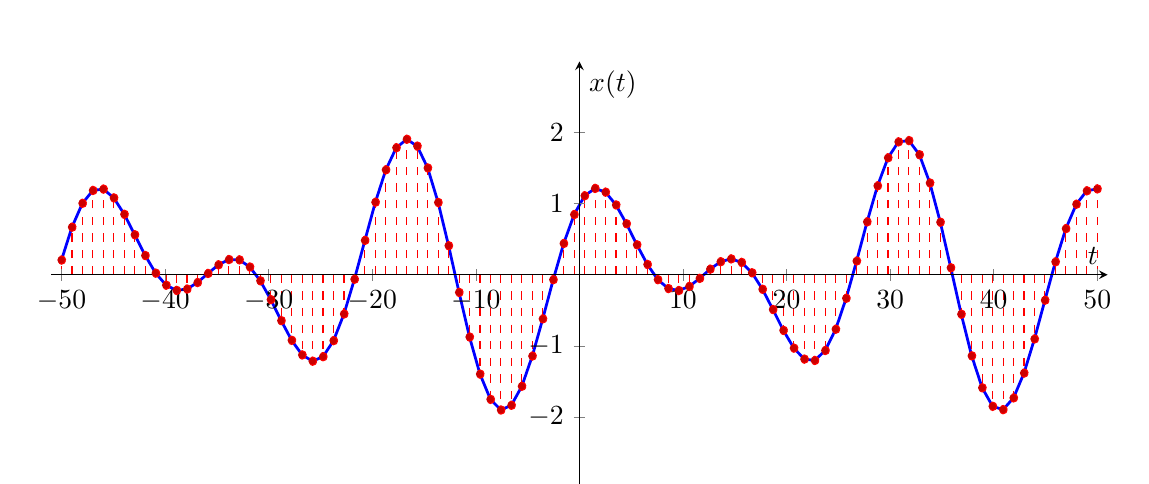
\begin{tikzpicture}
    \begin{axis}[xlabel=$t$, ylabel=$x(t)$, xmin=-51, xmax=51, ymin=-3, ymax=3,
    axis lines=center, axis on top=true, width=15cm,height=7cm,
    xtick={-50,-40,-30,-20,-10,10,20,30,40,50},
    ytick={-2,-1,1,2},
    mark size=1.5pt,
    ]
    \addplot[blue,line width=1pt] plot[domain=-50:50, samples=100]
    expression{sin(180*x/12)+cos(180*x/8)};
    \addplot+[ycomb,mark=*,red,dashed] plot[domain=-50:50, samples=100]
    expression{sin(180*x/12)+cos(180*x/8)};
   
    \end{axis}
    \end{tikzpicture}
    \caption{Talasni oblik uzorkovanog i izvornog analognog signala}
    \label{Sličica 1}
    
\end{figure}

\begin{figure}[!htb]
\begin{minipage}[b]{0.5\linewidth}\centering
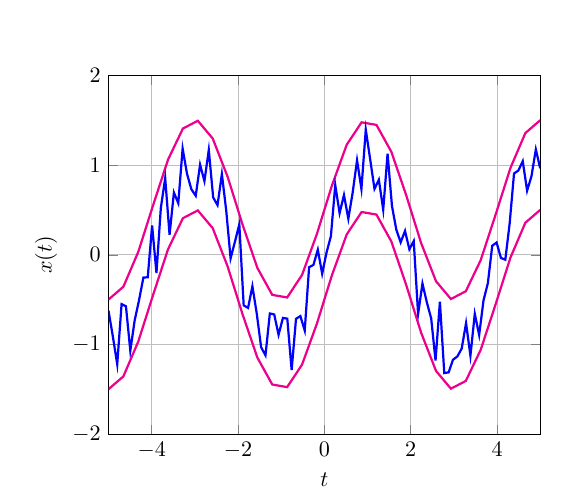
\begin{tikzpicture}[scale=0.8]
\begin{axis}[xlabel=$t$,ylabel= $x(t)$,grid=major,xmin=-5,xmax=5,ymin=-2,ymax=2]
\plot[magenta,line width=1pt] plot[domain=-5:5,samples=30] expression{sin(90*x)+0.5};
\plot[blue,line width=1pt] plot[domain=-5:5,samples=100] expression{sin(90*x)+0.4*rand};
\plot[magenta,line width=1pt] plot[domain=-5:5,samples=30] expression{sin(90*x)-0.5};
\end{axis}
\end{tikzpicture}
\caption{Sinusne funkcije sa i bez obličenja}
\label{Sličica 2}
\end{minipage}
{}
\begin{minipage}[b]{0.5\textwidth}\centering
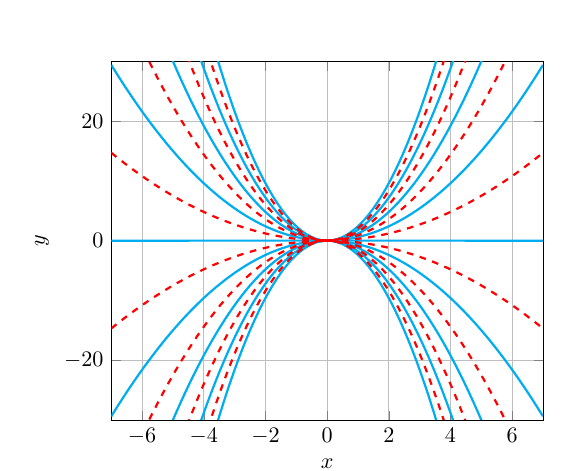
\begin{tikzpicture}[scale=0.8]
\begin{axis}[grid=major, xmin=-7,xmax=7,ymin=-30,ymax=30, xlabel=$x$,ylabel=$y$]		
\foreach \a in{-2.4,-1.8,...,2.4}{
\addplot[cyan,line width=1pt] plot[domain=-7:7, samples=100]
expression{\a*x^2};}
\foreach \a in{-2.1,-1.5,-0.9,-0.3,0.3,0.9,1.5,2.1}{
\addplot[red,line width=1pt,dashed] plot[domain=-7:7, samples=100]
expression{\a*x^2};}
\end{axis}
\end{tikzpicture}
\caption{Serija parabola}
\label{Sličica 3}
\end{minipage}
\end{figure}

\vspace{5mm}
Na slici \ref{Sličica 3} prikazana je serija parabola oblika $y = ax^2$ kreiranih sa okruženjem \plavo{tikzpicture} i \plavo{axis} . Ser-ija parabola nacrtana je za opseg vrijednosti $a =$ \{$−2.4, −2.1, ..., 2.4$\}. Za crtanje serije parabola koristiti komandu \color{mycolor1}\textbackslash{}\texttt{addplot}\color{black}\{\} u sklopu komande \color{mycolor1}\textbackslash{}\texttt{foreach}\color{black}\{\} koja ima varijablu \textbf{a} koja se mijenja u skladu sa prethodno definiranim opsegom i korakom. Obratiti pažnju da su neke krive markirane sa crvenom bojom (isprekidana linija) a neke plavom\footnote[6]{Obratiti pažnju na boje kao i njihove nijanse, u dokumentu.}.

\subsection{Električne, blok sheme i {\color{mycolor1}\textsl{circuitikz}} paket}
Na slici \ref{Sličica 4} prikazana je implementacija duo-binarnog registra sa SR FF\footnote[7]{Prilikom crtanja logičke sheme neophodno je uključiti \textit{tikz} bibllioteku \textit{circuits.logic.US} \vspace{35mm}}.\space Ukoliko imate poteškoća sa real-izacijom logičke i električne sheme, možete se poslužiti primjerima iz kratkog \textsl{manuala} \texttt{circutikz} paketa, koje se nalazi na CTAN \href{http://texdoc.net/texmf-dist/doc/latex/circuitikz/circuitikzmanual.pdf}{\color{cyan}stranici}.

\newpage
\begin{figure}[!htb]
\begin{center}
\tikzset{flipflop/port label/.style={font=\small\textit}}
\tikzset{flipflop SR/.style={flipflop,,
flipflop def={t1=\textit{S}, t3=\textit{R}, t6=\textit{Q}, t4={\ctikztextnot{$Q$}},
td={}, nd=1, t2=\textit{CP},width=1.3}
 }}
\tikzstyle{branch}=[fill,shape=circle,minimum size=4pt,inner sep=0pt]
\begin{tikzpicture}[circuit logic US,every circuit symbol/.style={thick}]
    \node (x0) at (0,0){};
    \node (x1) at (0,-4){};
    \node[not gate,point down,inputs={n}](not1) at (1,-0.7){};
    \node[and gate, draw, logic gate inputs={nn}](and1) at (2.5,-0.1){};
    \node[and gate, draw, logic gate inputs={nn}](and2) at (2.5,-1.4){};
    \node[flipflop SR,scale=0.8](ff1) at (5,-0.75)  {};
    \draw(5,0.25) node[above]{\scriptsize{SR-FF}};
    \node[flipflop SR,scale=0.8](ff2) at (5,-4.75) {};
    \draw(5,-3.75) node[above]{\scriptsize{SR-FF}};
    \node[not gate,point down,inputs={n}](not2) at (1,-4.7){};
    \node[and gate, draw, logic gate inputs={nn}](and3) at (2.5,-4.1){};
    \node[and gate, draw, logic gate inputs={nn}](and4) at (2.5,-5.4){};
    \draw (x0) node[below]{\scriptsize{$a_{0}$}}-- (and1.input 1);
    \draw (not1.input) --(1,0) node[branch]{};
    \draw (and1.output)--(ff1.pin 1);
    \draw (and2.output)--(ff1.pin 3);
    \draw (not1.output)|-(and2.input 2);
    \draw (and1.input 2) -|(1.6,-6.4)node[below]{\scriptsize{ENABLE}};
    \draw (and2.input 1)--(1.6,-1.3) node[branch]{};
    \draw (x1) node[below]{\scriptsize{$a_1$}} --(and3.input 1);
    \draw (not2.input)--(1,-4) node[branch]{};
    \draw (and3.output)--(ff2.pin 1);
    \draw (and4.output)--(ff2.pin 3);
    \draw (not2.output)|-(and4.input 2);
    \draw (and3.input 2)--(1.6,-4.2) node[branch]{};
    \draw (and4.input 1)--(1.6,-5.3) node[branch]{};
    \draw (ff1.pin 2)-|(3.7,-6.4)node[below]{\scriptsize{CP}};
    \draw (ff2.pin 2)--(3.7,-4.75) node[branch]{};
    \draw (ff1.bdown)|-(5,-2.5)--(6.1,-2.5)|-(5,-6.1) node[branch]{};
	\draw (ff2.bdown)--(5,-6.4)node[below]{\scriptsize{RESET}};   
    \draw (ff1.pin 4) --([xshift=3mm]ff1.pin 4);
    \draw (ff1.pin 6) --([xshift=3mm]ff1.pin 6);
    \draw (ff2.pin 4) --([xshift=3mm]ff2.pin 4);
    \draw (ff2.pin 6) --([xshift=3mm]ff2.pin 6);
    
\end{tikzpicture}
\caption{Implementacija duo-binarnog registra sa SR FF}
\label{Sličica 4}
\end{center}
\end{figure} 
Na slici \ref{Sličica 5} prikazana je ekvivalentna shema jednog pojačavačkog stepen.\newtodo{{Upotrijebiti opciju \texttt{american} u okruženju \space \space \space{\color{blue}\texttt{circuitikz}}} za generisanje simbola prema američkom \space \space standardu označavanja elektroničkih komponenti.} U okviru električne sheme (na slici \ref{Sličica 5}) korištene su sljedeće komponente: \texttt{\small{R, L, C i american current source}}.

\begin{figure}[htb!]
\hspace{7mm}
\tikzstyle{branch}=[fill,shape=circle,minimum size=3.5pt,inner sep=0pt]
\begin{circuitikz}[american voltages, american resistors,>=latex']

\draw(0,2.6) to [open,v^=$u_{ul}$,o-o](0,0);
\draw (0,2.6) to [short,i_=$i_{ul}$](1.8,2.6);
\draw(0,2.6) to [short,-*](1.8,2.6)node[above]{A$_1$}to [R,l_=$R_{1}$,i>=$i_{_{2}}$] (4.5,2.6);
\draw(4.5,2.6)node[above]{B$_1$}to [C, l_=$C_{_{E1}}$, i>=$i_{e1}$, *-,color=tamnozelena](4.5,0);
\draw(4.5,0)to [R, l^=$R_{_{5}}$, i>=$i_{6}$, *-*](4.5,-2.6);
\draw(1.8,-2.6)to [american inductor=$L_{2}$,i>=$i_{_{5}}$,color=magenta] (4.5,-2.6);
\draw(10,0) node[branch]{} to(10,-2.6);
\draw(4.5,-2.6)  to [C=$C_{4}$,i>=$i_{_{7}}$,color=tamnozelena] (10,-2.6);
\draw (7,2.6) to [american current source,l=$gi_{1}$, color=orange](4.5,2.6) (7,2.6)--(7.5,2.6);
\draw (7.5,2.6) to [american inductor,l_=$L_1$, i>=$i_{_{4}}$,*-*,color=magenta] (7.5,0);
\draw (1.8,2.6) to [C,l^=$C_{_{1}}$, i>=$i_{_{1}}$,*-*,color=tamnozelena] (1.8,0);
\draw (1.8,0) to [R,l^=$R_{_{3}}$, i>=$i_{_{5}}$] (1.8,-2.6);
\draw (7.5,2.6)--(8.5,2.6);
\draw (8.9,2.6) to [open, v_=$u_{12}$] (8.9,0);
\draw (8,2.6) to [C,l_=$C_{C}$,-*, i>=$i_{C}$,color=tamnozelena] (10.8,2.6);
\draw (8,2.6) node[above]{D$_1$}(8.5,2.6);
\draw (10.8,0) node[below]{F$_1$}to [american current source,l=$hi_{2}$, color=orange] (10.8,2.6) node[above]{E$_1$};
\draw (8,0) to [short] (13.8,0);
\draw (12.5,2.6) to [R, l_=$Z_{E2}$] (12.5,0);
\draw (10.8,2.6) to [short] (13.8,2.6);
\draw (13,2.6) to [short,i_=$i_{iz}$] (13.2,2.6);
\draw (13.8,2.6) to [R, l_=$R_p$,color=cyan] (13.8,0);
\draw (14.2,2.6) to [open, v^=$u_{iz}$] (14.2,0);
\draw (12.5,2.6) to [short] (13.8,2.6);
\draw (0,0) to [short] (8,0);

\draw[->,rounded corners=5pt,color=blue,dashed]
(8.7,1.4)|-(13,2.2)--(13,0.4)--(8.7,0.4);
\draw[->,rounded corners=5pt,color=red]
(0.75,1.4)|-(4,2.2)--(4,0.4)--(0.75,0.4);

\node[align=left] at (12.5,-1.8) {$A_v=\frac{u_{iz}}{u_{ul}}$ \\ \\
$A_{vdB}=20\log\frac{u_{iz}}{u_{ul}}$};
\end{circuitikz}
\caption{Ekvivalentna shema hipotetičkog pojačavača}
\label{Sličica 5}
\end{figure}
Slika \ref{Sličica 6} predstavlja model jednog komunikacijskog sistema. Prilikom crtanja modela i ostalih \texttt{tikz} baziranih
dijagrama/graka/slika možete se poslužiti aplikacijama kao što je \textsl{ktikz, QTikZ, TpX, fredokun TikZ-Editor} i sl.

\newpage
\begin{figure}[!htb]
    \centering

\pgfdeclareradialshading{spheregreen1}{\pgfpoint{-0.8cm}{1cm}}%
{rgb(0cm)=(0.7980,0.9686,0.9255);
rgb(1.5cm)=(0.2412,0.3941,0.0392)
}

\pgfdeclareradialshading{spherered1}{\pgfpoint{-0.8cm}{1cm}}%
{rgb(0cm)=(0.9686, 0.3569,0.3647);
rgb(1.5cm)=(0.5176,0.0353,0.1216)
}

\pgfdeclareradialshading{spherered2}{\pgfpoint{-0.8cm}{1cm}}%
{rgb(0cm)=(0.9686, 0.7569,0.7647);
rgb(1.5cm)=(0.5176,0.1353,0.1216)
}

\pgfdeclareradialshading{spheregray1}{\pgfpoint{-0.8cm}{1cm}}%
{rgb(0cm)=(0.9537,0.9473,0.9373);
rgb(1.5cm)=(0.3843,0.2784,0.3960)
}

\pgfdeclareradialshading{spheregray2}{\pgfpoint{-0.8cm}{1cm}}%
{rgb(0cm)=(1,1,1);
rgb(7.5cm)=(0.2176,0.2392,0.1294)
}

\pgfdeclareradialshading{sphereblue1}{\pgfpoint{-0.8cm}{1cm}}%
{rgb(0cm)=(0.7137,0.7373,0.9373);
rgb(1.5cm)=(0.2314,0.1373,0.6431)
}
\pgfdeclareradialshading{sphereblue2}{\pgfpoint{-0.8cm}{1cm}}%
{rgb(0cm)=(0.7137,0.7373,0.9373);
rgb(1.5cm)=(0.5450,0.4470,0.6627)
}
\pgfdeclareradialshading{sphereyellow1}{\pgfpoint{-0.8cm}{1cm}}%
{rgb(0cm)=(0.9537,0.9473,0.9373);
rgb(1.5cm)=(0.937,0.941,0.682)
}

\tikzstyle{okvir} = [draw,rectangle,rounded corners=3pt, line width=0.5pt,gray]
\tikzstyle{blok1} = [draw,rectangle,minimum width=17mm,minimum height = 10mm, line width=0.5pt,rounded corners=2pt,gray,drop shadow]
\tikzstyle{blok2} = [draw,rectangle,minimum width=19mm,minimum height = 10mm, line width=0.5pt,rounded corners=2pt,gray,drop shadow]
\tikzstyle{blok3} = [draw,rectangle,minimum width=18mm,minimum height = 10mm, line width=0.5pt,rounded corners=2pt,gray,drop shadow]
\tikzstyle{blok4} = [draw,rectangle,minimum width=20mm,minimum height = 10mm, line width=0.5pt,rounded corners=2pt,gray,drop shadow]
\tikzstyle{input} = [coordinate]
\begin{tikzpicture}     

\draw[rounded corners=5pt,color=gray,dashed]
(0,0)-|(16,-4.5)-|(0,0);

\draw node[anchor=west,xshift=15mm,yshift=-15mm,okvir,minimum height=16mm,minimum width=48mm,shading=spheregray2](b00){}; 
 
\draw (2.6,-1.4) node[blok3, shading=sphereblue1](b0){}; 
\draw (b0) node[yshift=2mm]{\color{white}\sffamily\tiny\textbf{TURBO}};
\draw (b0) node[yshift=0mm]{\color{white}\sffamily\tiny\textbf{KONVOLUCIONI}};
\draw (b0) node[yshift=-2mm]{\color{white}\sffamily\tiny\textbf{KODER}};

\draw (b0.east) node[anchor=west,xshift=6mm,blok2,shading=spheregreen1](b1){};
\draw (b1) node[yshift=2mm]{\color{white}\sffamily\tiny\textbf{VIŠESTRUKI}};
\draw (b1) node[yshift=0mm]{\color{white}\sffamily\tiny\textbf{REPLIKATOR BITA}};
\draw (b1) node[yshift=-2mm]{\color{white}\sffamily\tiny\textbf{ZAGLAVLJA PAKETA}};

\draw (b1.east) node[anchor=west,xshift=23mm,blok3,shading=spheregray1](b2){};
\draw (b2) node[yshift=0mm]{\color{white}\sffamily\tiny\textbf{MAPER}};

\draw (b2.east) node[anchor=west,xshift=7mm,blok4,shading=spherered2](b3){};
\draw (b3) node[yshift=3mm]{\color{white}\sffamily\tiny\textbf{PRIMJENA}};
\draw (b3) node[yshift=1mm]{\color{white}\sffamily\tiny\textbf{TONSKE MASKE}};
\draw (b3) node[yshift=-1mm]{\color{white}\sffamily\tiny\textbf{AMPLITUDNE MASKE}};
\draw (b3) node[yshift=-3mm]{\color{white}\sffamily\tiny\textbf{INVERZNE FFT 4096}};

\draw (b3.east) node[anchor=west,xshift=7mm,blok4,shading=spherered1](b4){};
\draw (b4) node[yshift=3mm]{\color{white}\sffamily\tiny\textbf{DODAVANJE}};
\draw (b4) node[yshift=1mm]{\color{white}\sffamily\tiny\textbf{CIKLIČNOG PREFIKSA}};
\draw (b4) node[yshift=-1mm]{\color{white}\sffamily\tiny\textbf{UOBLIČAVANJE I}};
\draw (b4) node[yshift=-3mm]{\color{white}\sffamily\tiny\textbf{PREKLAPANJE}};

\draw node[anchor=west,xshift=15mm,yshift=-34mm,okvir,minimum height=16mm,minimum width=72mm,shading=sphereyellow1](b01){};

\draw (2.6,-3.35) node[blok3,shading=sphereblue2](b5){};
\draw (b5) node[yshift=1mm]{\color{white}\sffamily\tiny\textbf{PSEUDOSLUČAJNI}};
\draw (b5) node[yshift=-1mm]{\color{white}\sffamily\tiny\textbf{KODER}};

\draw (b5.east) node[anchor=west,xshift=7mm,blok1,shading=sphereblue1](b6){};
\draw (b6) node[yshift=2mm]{\color{white}\sffamily\tiny\textbf{TURBO}};
\draw (b6) node[yshift=0mm]{\color{white}\sffamily\tiny\textbf{KONVOLUCIONI}};
\draw (b6) node[yshift=-2mm]{\color{white}\sffamily\tiny\textbf{KODER}};

\draw (b6.east) node[anchor=west,xshift=7mm,blok3,shading=spheregreen1](b7){};
\draw (b7) node[yshift=1mm]{\color{white}\sffamily\tiny\textbf{KANALANI}};
\draw (b7) node[yshift=-1mm]{\color{white}\sffamily\tiny\textbf{PREPLETAČ}};

\draw [->,>=latex'](1,-1.4)--(b0);
\draw[->,>=latex'] (b0)--(b1);
\draw[->,>=latex'] (b1)--(b2); 
\draw[->,>=latex'] (b2)--(b3);
\draw[->,>=latex'] (b3)--(b4); 
\draw[->,>=latex'] (1,-3.35)--(b5);
\draw[->,>=latex'] (b5)--(b6); 
\draw[->,>=latex'] (b6)--(b7); 
\draw[->,>=latex'] (b7)-|(b2);

\draw[rounded corners=5pt,color=gray,dashed]
(0,-6.1)-|(16,-10.5)-|(0,-6.1);

\draw (2,-7.35) node[blok1, shading=spherered2](b8){}; 
\draw (b8) node[yshift=1mm]{\color{white}\sffamily\tiny\textbf{AGC}};
\draw (b8) node[yshift=-1mm]{\color{white}\sffamily\tiny\textbf{FFT 4096}};

\draw (b8.east) node[anchor=west,xshift=7mm,blok1,shading=spheregray1](b9){};
\draw (b9) node[yshift=0mm]{\color{white}\sffamily\tiny\textbf{DEMODULATOR}};

\draw (b9.east) node[anchor=west,xshift=6mm,yshift=-1mm,okvir,minimum height=16mm,minimum width=48mm,shading=spheregray2](b03){};

\draw (b9.east) node[anchor=west,xshift=8mm,blok2,shading=spheregreen1](b10){};
\draw (b10) node[yshift=2mm]{\color{white}\sffamily\tiny\textbf{KOMBINIRANJE}};
\draw (b10) node[yshift=0mm]{\color{white}\sffamily\tiny\textbf{KOPIJA BITA}};
\draw (b10) node[yshift=-2mm]{\color{white}\sffamily\tiny\textbf{ZAGLAVLJA PAKETA}};

\draw (b10.east) node[anchor=west,xshift=7mm,blok1,shading=sphereblue1](b11){};
\draw (b11) node[yshift=2mm]{\color{white}\sffamily\tiny\textbf{TURBO}};
\draw (b11) node[yshift=0mm]{\color{white}\sffamily\tiny\textbf{KONVOLUCIONI}};
\draw (b11) node[yshift=-2mm]{\color{white}\sffamily\tiny\textbf{DEKODER}};

\draw (b03.south) node[anchor=north,xshift=12mm,yshift=-2mm,okvir,minimum height=16mm,minimum width=72mm,shading=sphereyellow1](b04){};

\draw (b10.south) node[anchor=north,yshift=-8mm,okvir,blok3,shading=spheregreen1](b12){};
\draw (b12) node[yshift=2mm]{\color{white}\sffamily\tiny\textbf{INVERZNI}};
\draw (b12) node[yshift=0mm]{\color{white}\sffamily\tiny\textbf{KANALNI}};
\draw (b12) node[yshift=-2mm]{\color{white}\sffamily\tiny\textbf{PREPLETAČ}};

\draw (b12.east) node[anchor=west,xshift=7mm,blok3,shading=sphereblue1](b13){};
\draw (b13) node[yshift=2mm]{\color{white}\sffamily\tiny\textbf{TURBO}};
\draw (b13) node[yshift=0mm]{\color{white}\sffamily\tiny\textbf{KONVOLUCIONI}};
\draw (b13) node[yshift=-2mm]{\color{white}\sffamily\tiny\textbf{DEKODER}};

\draw (b13.east) node[anchor=west,xshift=7mm,blok3,shading=sphereblue2](b14){};
\draw (b14) node[yshift=1mm]{\color{white}\sffamily\tiny\textbf{PSEUDOSLUČAJNI}};
\draw (b14) node[yshift=-1mm]{\color{white}\sffamily\tiny\textbf{DEKODER}};

\draw[->,>=latex'] (b8)--(b9); 
\draw[->,>=latex'] (b9)--(b10);
\draw[->,>=latex'] (b10)--(b11);
\draw[->,>=latex'] (b11)--(14.2,-7.35);
\draw[->,>=latex'] (b9)|-(b12);
\draw[->,>=latex'] (b12)--(b13);
\draw[->,>=latex'] (b13)--(b14);
\draw[->,>=latex'] (b14)--(14.2,-9.15);

\draw (b00.north west) node[anchor= south east,xshift=25mm,yshift=1mm]{\sffamily\small\textbf{IEEE P1901 PREDAJNIK}};
\draw (b03.south west) node[anchor= north east,xshift=-18mm,yshift=-17mm]{\sffamily\small\textbf{IEEE P1901 PREDAJNIK}};
\draw (b0.south) node[anchor=north,xshift=11mm,yshift=-0.5mm]{\sffamily\tiny\textbf{P1901 KANALNI KODER KONTROLNIH PODATKA}};
\draw (b5.south) node[anchor=north,xshift=10mm]{\sffamily\tiny\textbf{P1901 KANALNI KODER KORISNIH PODATAKA}};
\draw (b10.south) node[anchor=north,xshift=12mm,yshift=-0.5mm]{\sffamily\tiny\textbf{1901 KANALNI DEKODER KONTROLNIH PODATAKA}};
\draw (b12.south) node[anchor=north,xshift=11mm,yshift=-0.5mm]{\sffamily\tiny\textbf{P1901 KANALNI DEKODER KORISNIH PODATAKA}};

\draw [color=black,line width=1.5pt](0,-5.3)--(8,-5.3) node[above]{\small\textbf{Energetski kabl}}--(16,-5.3);
\draw[->,>=latex'] (b4)--++(down:39mm);
\draw[<-,>=latex'] (b8)--++(up:20.5mm);

\draw (b0.west) node[anchor=north east,xshift=-2.5mm,yshift=0.5mm]{\sffamily\tiny\textbf{Kontrolni}};
\draw (b0.west) node[anchor=north east,xshift=-3.5mm,yshift=-1.5mm]{\sffamily\tiny\textbf{podaci}};
\draw (b5.west) node[anchor=north east,xshift=-3.5mm,yshift=0.5mm]{\sffamily\tiny\textbf{Korisni}};
\draw (b5.west) node[anchor=north east,xshift=-3.5mm,yshift=-1.5mm]{\sffamily\tiny\textbf{podaci}};
\draw (b11.east) node[anchor=west,xshift=37mm,yshift=1mm]{\sffamily\tiny\textbf{Kontrolni}};
\draw (b11.east) node[anchor=west,xshift=37mm,yshift=-1mm]{\sffamily\tiny\textbf{podaci}};
\draw (b14.east) node[anchor=west,xshift=11.5mm,yshift=1mm]{\sffamily\tiny\textbf{Korisni}};
\draw (b14.east) node[anchor=west,xshift=11.5mm,yshift=-1mm]{\sffamily\tiny\textbf{podaci}};

    \end{tikzpicture}
    \caption{Primjer modela komunikacijskog sistema}
    \label{Sličica 6}
\end{figure}

\vfill{}
\hfill{}\color{red}Sretno \color{blue}kodiranje!

\end{document}